\textbf{Ejemplo 1}\\

Dos ciudades A y B están unidos mediante una vieja carretera y se proyecta la construcción de una nueva carretera que costará  100 millones COP y que acortará el camino entre éstas dos ciudades. Esto implica una disminución en el consumo del combustible, aceites, desgaste de vehículos y en el valor del peaje. Todas estas disminuciones se estiman que pueden llegar a valer 28 millones COP al año. Por otra parte, hay varios comerciantes que han montado restaurantes y hoteles a lo largo de la carretera antigua y con la construcción de la nueva carretera el perjuicio que recibirán estos por la disminución del turismo, ascendería a  15 millones COP al año. Utilizando la Relación B/C determinar la conveniencia del proyecto utilizando: a) una tasa del 30\% pav y b) tasa del 12\% pav.


Comentario: La disminución en consumo de combustibles, aceites, desgaste de
vehículos y disminución de peajes vienen a ser un beneficio y la pérdida de turismo viene
a ser un desbeneficio porque en ambos casos es el público el que recibe las consecuencias, mientras que el valor del proyecto es el costo cuyo desembolso la hace el estado.
\\

\textbf{Solución.}\\

El CAUE (Costo Anual Unificado Equivalente) de los beneficios y los perjuicios es igual a 28 millones COP - 15 millones COP = 13 millones COP. El CUAE del costo del proyecto lo podemos calcular asumiendo que los 100 millones COP corresponden al valor presente de una serie infinita de \$ X c/u al final de cada año.
%La tabla ira centrada
\begin{center}
	\renewcommand{\arraystretch}{1.5}% Margenes de las celdas
	%Creación de la cuadricula de 3 columnas
\begin{longtable}[H]{|c|c|c|}
		%Creamos una linea horizontal
\hline
		%Definimos el color de la primera fila
\rowcolor[HTML]{FFB183}
	%%%%% INICIO ASIGNACIÓN PERÍODO FOCAL %%%%%%%
  %%%%%%%%%% INICIO TITULO
  %Lo que se hace aquí es mezclar las 3 columnas en una sola
  \multicolumn{3}{|c|}{\cellcolor[HTML]{FFB183}\textbf{1. Asignación período focal}}   \\ \hline
  %%%%%%%%%% FIN TITULO
  %%%%% INICIO DECLARACIÓN DE VARIABLES %%%%%%%
  \multicolumn{3}{|c|}{$pf :0 pav$}   \\ \hline
  %%%%% INICIO DECLARACIÓN FORMULAS
  
%%%%%%%%%%% INICIO TITULO
\rowcolor[HTML]{FFB183}
\multicolumn{3}{|c|}{\cellcolor[HTML]{FFB183}\textbf{2. Declaración de variables}}    \\ \hline
\multicolumn{1}{|c|}{\cellcolor[HTML]{FFB183}\textbf{Valores monetarios}}    & \multicolumn{1}{c|}{\cellcolor[HTML]{FFB183}\textbf{Valores no monetarios}} & \multicolumn{1}{c|}{\cellcolor[HTML]{FFB183}\textbf{Incógnitas}} \\ \hline
%%%%%%%%%%% FIN TITULO
%%%%%%%%%%% INICIO MATEMÁTICAS

$ Ingresos =     28 \text{ millones COP} $  &  {$ i_a = 30\% pav $}  & { $ VPN =    ?   COP $ }\\
$ Egresos =     15 \text{ millones COP} $  &  {$ i_b = 12\% pav $}  & { $ \frac{B}{C_a} =    ?   \% $ } \\ 
$ VP = \text{100 millones COP}$     &&  { $ \frac{B}{C_b} =    ?   \% $ } \\
$ $	                                                         &  &{ $ R_a =    ?   COP $ } \\ 
$ $	                                                         &  &{ $ R_b =    ?   COP $ } \\ 

\hline
%%%%%%%%%% FIN MATEMÁTICAS
		%%%%% INICIO FLUJO DE CAJA
\rowcolor[HTML]{FFB183}
\multicolumn{3}{|c|}{\cellcolor[HTML]{FFB183}\textbf{3. Diagrama de flujo de caja}} \\ \hline
		%Mezclamos 3 columnas y pondremos el dibujo
		%%%%%%%%%%%%% INSERCIÓN DE LA IMAGEN
		%Deberán descargar las imágenes respectivas del drive y pegarlas en la carpeta
		%n_capitulo/img/ejemplos/1/capitulo1ejemplo1.pdf  (el /1/ es el numero del ejemplo)
\multicolumn{3}{|c|}{ 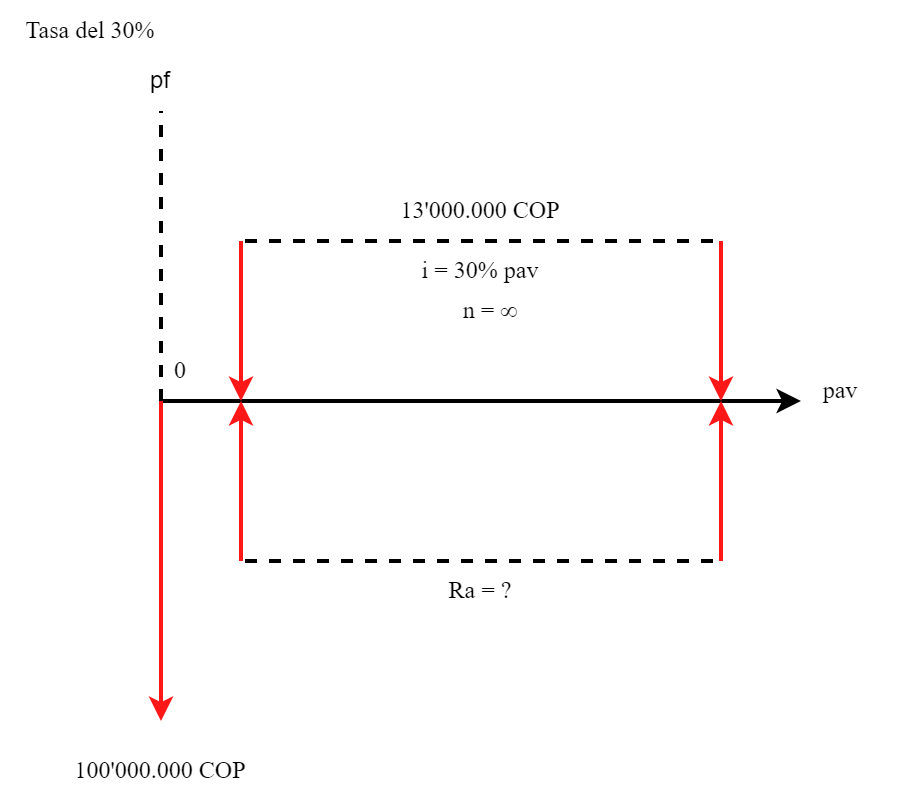
\includegraphics[width=10.5cm]{EJ12_1A.png}}   
\\
\multicolumn{3}{|c|}{ 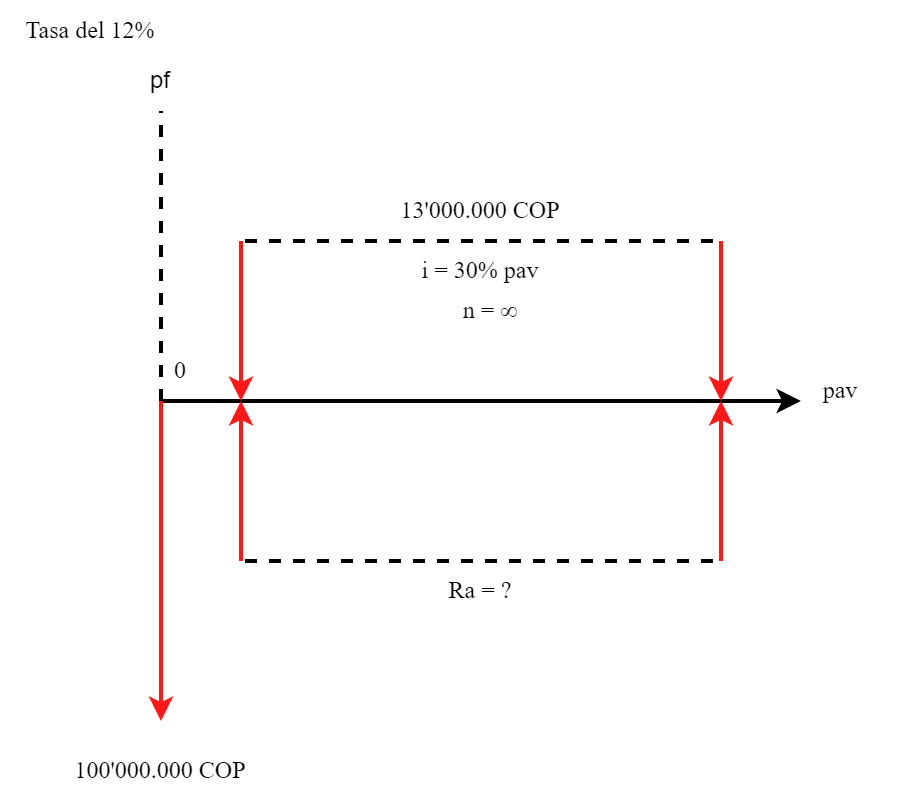
\includegraphics[width=10.5cm]{EJ12_1B.png}}   
   \\ \hline
		%%%%%%%%%%%%% FIN INSERCIÓN DE IMAGEN
		%%%%%FIN FLUJO DE CAJA
		
		
		
		%%%%% INICIO DECLARACIÓN FORMULAS
		%%%%%%%%%%% INICIO TITULO
\rowcolor[HTML]{FFB183}
\multicolumn{3}{|c|}{\cellcolor[HTML]{FFB183}\textbf{4. Declaración de fórmulas}}    \\ \hline
		%%%%%%%%%%% FIN TITULO
		%%%%%%%%%%% INICIO MATEMÁTICAS
\multicolumn{3}{|c|} {$VPN = \Sigma(Costos) - \Sigma(Inversiones) $\hspace{15pt}\textit{Valor Presente Neto}}   \\ 
\multicolumn{3}{|c|} {$VP = \frac{R}{i}$\hspace{15pt}\textit{ Valor Presente para una Serie Perpetua Vencida}}   \\ 
\multicolumn{3}{|c|} {$B/C = \frac{VPN}{VPC}$\hspace{15pt}\textit{ Relación Beneficio/Costo}}   \\ 
\hline	
	
		%%%%%%%%%% FIN MATEMÁTICAS
		%%%%%% INICIO DESARROLLO MATEMÁTICO
\rowcolor[HTML]{FFB183}
		%%%%%%%%%%INICIO TITULO
\multicolumn{3}{|c|}{\cellcolor[HTML]{FFB183}\textbf{5. Desarrollo matemático}}       \\ \hline
		%%%%%%%%%% FIN TITULO
		%%%%%%%%%% INICIO MATEMÁTICAS
		\multicolumn{3}{|c|}{$\quad \quad \quad \quad \quad \quad \text{ VPN = 28 millones COP - 15 millones COP =13 millones COP} \quad \quad \quad \quad \quad \quad $}  
		\\
		
		\multicolumn{3}{|c|}{$ R_a = (100 millones COP)(0.3) =    30 millones COP $}  
		\\
	
		\multicolumn{3}{|c|}{$ \frac{B}{C_a} = \frac{13}{30} = 0.43 < 1 $}
		\\ 
		\multicolumn{3}{|c|}{$ VPN_a = -100 + 13/0.3 = -  50.07 millones COP <0 $}
		\\ 
		\multicolumn{3}{|c|}{$ R_b =  (100 millonesCOP) (0.12) =   12 millones COP $}
		\\ 
		\multicolumn{3}{|c|}{$ \frac{B}{C_b} = \frac{13}{12} = 1.083 > 1 $}
		\\ 
		\multicolumn{3}{|c|}{$ VPN_b = -100 + 13/0.12 = 8.3 millones COP >0  $}
		\\ 
		\hline
				
		%%%%%%%%%% FIN MATEMÁTICAS
		%%%%%% FIN DESARROLLO MATEMÁTICO
		%%%%%% INICIO RESPUESTA
\rowcolor[HTML]{FFB183}
		%%%%%%%%%%INICIO TITULO
\multicolumn{3}{|c|}{\cellcolor[HTML]{FFB183}\textbf{6. Respuesta}}   \\ \hline
		%%%%%%%%%% FIN TITULO
		%%%%%%%%%% INICIO RESPUESTA MATEMÁTICA
  \multicolumn{3}{|c|}{ \text{Se recomienta hacer el proyecto con la tasa del 12\% pav } } \\ 
\multicolumn{3}{|c|}{ \text{  ya que la relacion B/C es mayor a 1 y el VPN lo confirma.} } \\ 
\hline		
		
		%%%%%%%%%% FIN MATEMÁTICAS
		%%%%%% FIN RESPUESTA
	\end{longtable}
	%Se crean dos lineas en blanco para que no quede el siguiente texto tan pegado
	%\newline \newline %USARLO SI CREES QUE ES NECESARIO
\end{center}
%%%%%%%%%%%%%%%%%%%%%%%%%%FIN EJERCICIO 1 %%%%%%%%%%%%%%%%%%%%%%%%%%%
